\documentclass[letterpaper]{article}
\usepackage[utf8]{inputenc}
\usepackage{url}
\usepackage{aaai}
\usepackage{times}
\usepackage{helvet}
\usepackage{courier}
\usepackage{amsmath}
\usepackage{amssymb}
\usepackage{graphicx}

% \frenchspacing
\setlength{\pdfpagewidth}{8.5in}
\setlength{\pdfpageheight}{11in}
\pdfinfo{
/Title (Temperature-Dependent Estimation of Vehicle Fuel Economy: Experimental Methodology)
/Author (Sindu Chitraju, Samuel Howard, Seif Ilkbarieh, Om Solanki, Andrew Wheeler)}
\setcounter{secnumdepth}{0}  

\begin{document}

% The file aaai.sty is the style file for AAAI Press 
% proceedings, working notes, and technical reports.

% Remove the copyright from the footer
\nocopyright

\title{Temperature-Dependent Estimation of Vehicle Fuel Economy:\\Experimental Methodology}
\author{Sindu Chitraju, Samuel Howard, Seif Ilkbarieh, Om Solanki, Andrew Wheeler\\
Tennessee Technological University
}

\maketitle

\section*{Our Dataset}
This project studies the predictive performance of recurrent neural network 
models on vehicle telemetry data, with a particular focus on how external 
and derived features works such as weather conditions, smoothed signals, 
and road grade that are influence by the accuracy of fuel consumption 
estimation. To conduct this study, we created multiple variants of the 
dataset and trained models under controlled conditions to remove the 
effects of each feature group.

The raw data used in this project was collected through the Torque mobile 
application, which logs real-time vehicle sensor data. These logs were 
cleaned and processed using a custom script \verb|(clean_data.py)| to ensure 
consistency and usability for machine learning. But only essential 
features such as engine RPM, throttle position, fuel usage, speed, 
altitude, and positional coordinates were retained. Duplicate entries were 
removed, and invalid/corrupted values, particularly those found in the fuel 
usage field, were filtered out. Instant fuel consumption values were pulled 
by computing the difference between successive readings of the cumulative 
trip fuel usage. The terrain slope, referred to as grade, was calculated 
using changes in altitude and vehicle speed, while its first derivative, 
``grade break,'' was included to reflect shifts in road incline. 
Historical weather data was integrated into the dataset using the 
Open-Meteo API, with temperature values mapped to each GPS coordinate 
and timestamp. In some versions of the dataset, a moving average filter 
was applied to smooth the time-series data and reduce the impact of sensor 
noise.

\section*{Dataset Attributes}

\subsection*{Vehicular Factors}

From our dataset, a few key metrics emerged concerning fuel consumption. 
The most obvious correlation is speed. As speed increases, drag increases 
with the square of velocity according to the equation: 
\[
    \displaystyle F_{\mathrm {D} }\,=\,{\tfrac {1}{2}}\,\rho \,v^{2}\,C_{\mathrm {D} }\,A
\] 

This, along with the peak efficiency of internal combustion engines (ICE), 
leads to a peak fuel economy that is generally found between 45 and 55 MPH. 
In our data, this peak is at roughly 50 MPH, as shown in Figure \ref{fig:mpgspeed}. 
As seen in Figure \ref{fig:histmpgspeed}, the amount of data we have drops off sharply 
past 60 MPH, 5 MPH above the common speed limit of highways in the United 
States.

% speed_vs_mpg.png figure
\begin{figure}[htbp]
    \centering
    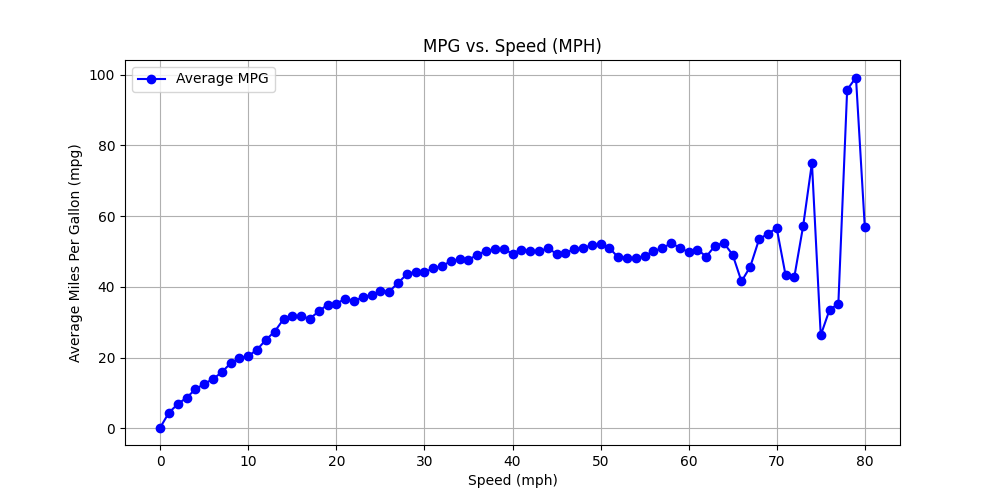
\includegraphics[width=0.5\textwidth]{figures/speed_vs_mpg.png}
    \caption{Plot of speed vs MPG}
    \label{fig:mpgspeed}
\end{figure}

% histogram_speedobdmph.png figure
\begin{figure}[htbp]
    \centering
    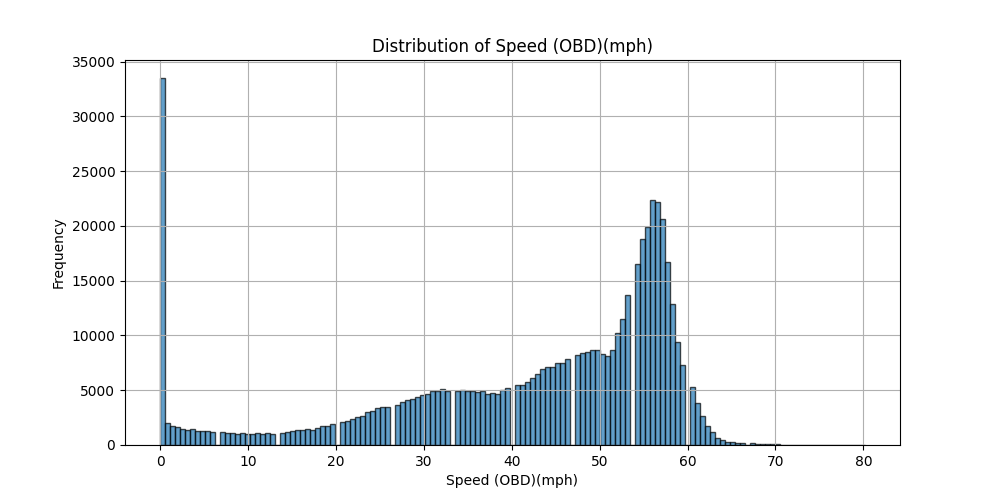
\includegraphics[width=0.5\textwidth]{figures/histogram_speedobdmph.png}
    \caption{Histogram of speed}
    \label{fig:histmpgspeed}
\end{figure}

Next on the list is temperature. The primary effect this has on fuel 
consumption is the density of the air entering the engine. Warmer air is 
less dense than colder air, leading to a decrease in fuel consumption as 
the Engine Control Unit (ECU) attempts to maintain a stoichiometric 
Air-Fuel Ratio (AFR) of roughly 14.7:1. However, warmer air comes with the 
issue of knock at the upper end of the temperature range. This is from the 
preignition of fuel in the combustion chamber before it is ignited by the 
spark plugs. To compensate for this, the ECU will delay ignition timing and 
even enrich the air-fuel mixture, leading to increased fuel consumption. 
Figure \ref{fig:intakeairtempmpg} shows this with a rapid decrease in fuel 
economy past an intake air temperature of approximately 100\textdegree F.

% intake_air_temp_mpg.png figure
\begin{figure}[htbp]
    \centering
    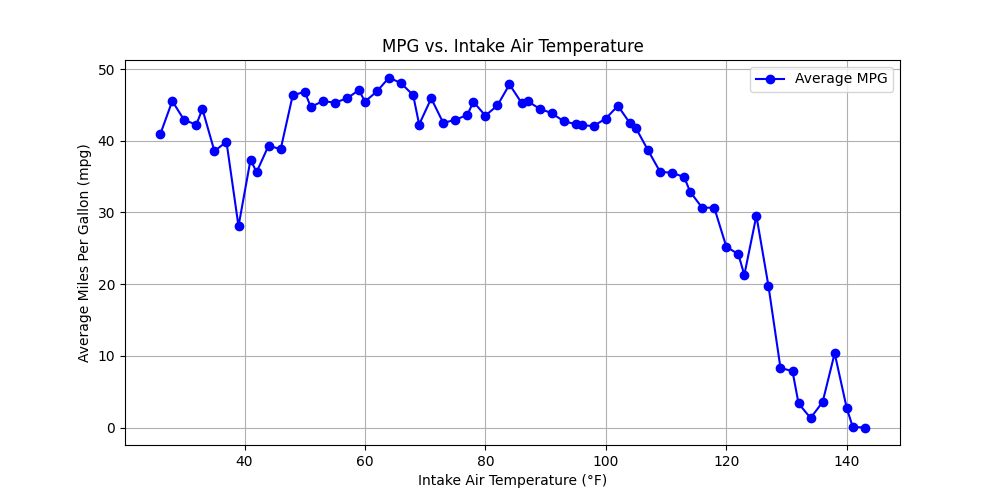
\includegraphics[width=0.5\textwidth]{figures/intake_air_temp_mpg.png}
    \caption{Intake Air Temperature (\textdegree F) vs MPG}
    \label{fig:intakeairtempmpg}
\end{figure}

Related to the temperature of the air coming in is the amount coming in. 
This is determined by the position of the throttle valve. In our case, two 
other factors come into play for the volumetric efficiency of the engine 
for a given throttle position that are a part of Honda's Variable Valve 
Timing and Lift Electronic Control system (VTEC). The iteration of the 
system used in the R18A1 engine of the test vehicle includes two methods 
to additionally control the volume and speed of air entering the engine: 
an additional set of camshaft lobes with lower lift and different 
duration, and valves to change the length of the runners in the intake 
plenum. 

The additional set of camshaft lobes reduces the lift of the intake valves 
and reduces the time they are left open. Furthermore, they are set forward 
of the regular camshaft lobes such that the effective length of the 
engine's intake stroke is reduced. This somewhat mimics the Atkinson cycle 
by making the intake stroke slightly shorter than the power (expansion) 
stroke. The change in effective stroke length has the added benefit of 
improving volumetric efficiency when combined with the ability to further 
open the throttle valve while cruising under light engine loads between 
1,000 and 3,000 RPM, which reduces pumping losses.

At higher RPMs, valves within the intake plenum open to reduce their 
effective length. This has the effect of improving power at the expense 
of fuel economy. Consequently, our dataset contains less of this data, 
along with the fact that this happens at approximately 4500 RPM.

These factors combine for a spike in fuel economy from the throttle 
position most common for coasting with Deceleration Fuel Cutoff (DFCO) 
that sharply tapers off for cruising and acceleration throttle positions 
as shown in FIgure \ref{fig:throttlevsmpg}. 

% throttle_vs_mpg.png figure
\begin{figure}[htbp]
    \centering
    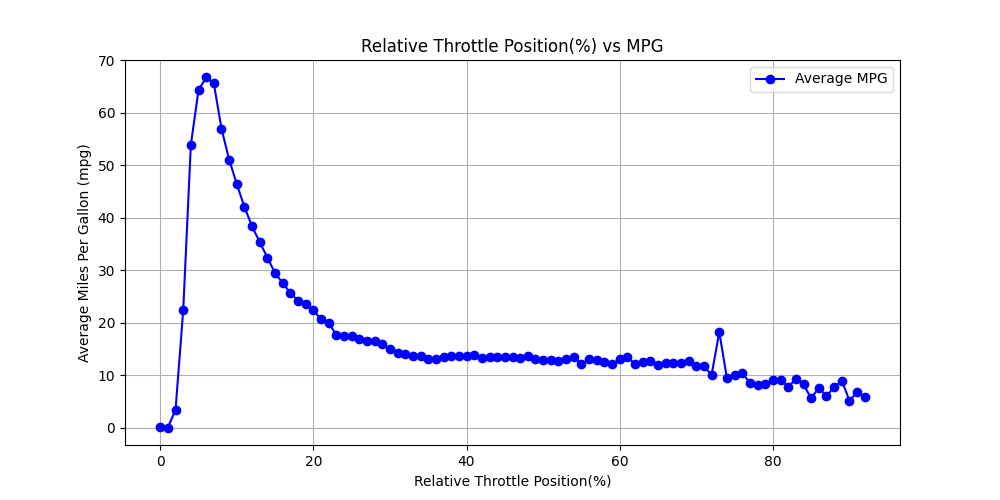
\includegraphics[width=0.5\textwidth]{figures/throttle_vs_mpg.png}
    \caption{Plot of throttle vs MPG}
    \label{fig:throttlevsmpg}
\end{figure}

\subsection*{Extravehicular Factors}

Weather, specifically temperature, was an additional chosen factor as it 
directly correlates with the intake air temperature and air density. It 
also changes less than the intake air temperature in traffic or other 
conditions where the vehicle is stopped. Finally, seasonal differences in 
fuel blends are dependent on cooler or warmer weather and can be accounted 
for along with the temperature.

Grade was the final factor added as it directly relates to the torque 
required to maintain a given speed (Figure \ref{fig:gradevsmpg}). Going up 
a hill increases this requirement, and going downhill reduces this 
requirement. This is not as important for the fuel economy result, but it 
is important for prediction along the route. We want to predict the fuel 
required to go up a hill, and how much (if any) it will take to go down it. 

\begin{figure}[htbp]
    \centering
    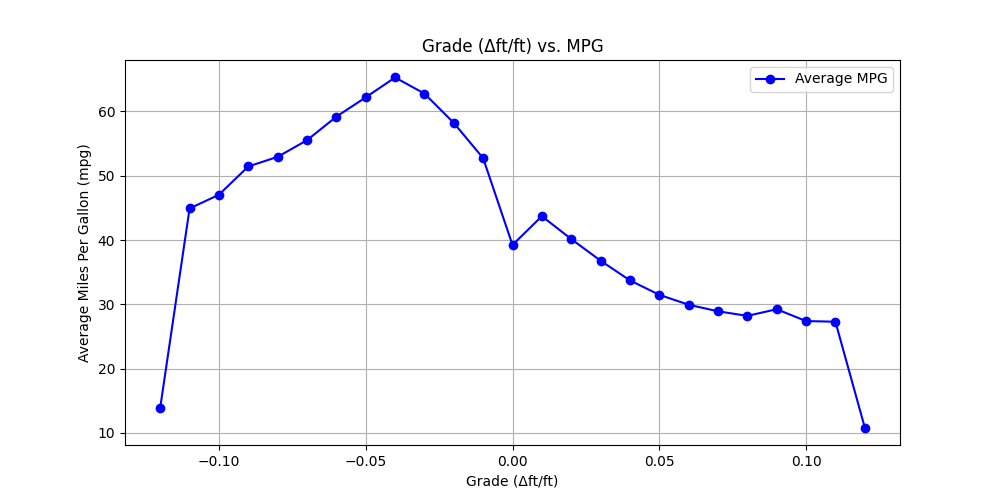
\includegraphics[width=0.5\textwidth]{figures/grade_vs_mpg.png}
    \caption{Plot of Grade vs MPG}
    \label{fig:gradevsmpg}
\end{figure}

\section*{Relation of Variables}

Many of the chosen variables are mathematically related to the fuel 
consumption of the engine by the following equation, where 
$V_{\mathrm{engine}}$ is the volume of the engine in Liters, $N$ is the 
RPM, $\dot{m}_{\mathrm{air}}$ is the air mass flow rate in kg/min, $14.7$ 
is the stochiometric ratio (:1) for a gasoline-air mixture, and $0.74$ is 
the density of gasoline in kg/L.

\[
\text{Fuel volume per minute (L/min)} = \cfrac{\frac{V_{\mathrm{engine}}}{2} \times N \times \dot{m}_{\mathrm{air}}}{14.7\times 0.74}
\]

For this reason, we have included RPM and intake air temperature as 
variables in our model. Related to this is brake-specific fuel consumption 
with the following formula, where $P_{\mathrm{brake}}$ is the brake power 
output of the engine in kilowatts (kW), $\dot{m}_{\mathrm{fuel}}$ is the 
flow rate of fuel in g/h.

\[
\mathrm{BSFC} = \cfrac{\dot{m}_{\mathrm{fuel}}}{P_{\mathrm{brake}}}
\]

Brake power is defined as follows, where $T$ is the torque in Newton-meters 
(Nm) and $9550$ is a constant for unit conversion.

\[
P_{\mathrm{brake}} = \cfrac{T \times N}{9550}
\]

Combining some more formulas, T is defined as follows, where $C_d$ is the 
drag coefficient, $A$ is the frontal area of the vehicle ($m^2$), $\rho$ 
is the air density in kg/m\textsuperscript{3}, $v$ is the vehicle speed 
in m/s, $C_{rr}$ is the coefficient of rolling resistance of the vehicle, 
$m$ is the mass of the vehicle in kg, $g$ is gravitational acceleration 
($\approx 9.81 \mathrm{m}/\mathrm{s}^2$), Grade is the slope of the road, 
and $R$ is the radius of the tire in(m).

\[
T = (\frac{1}{2}C_d\times A \times \rho \times v^2 + C_{rr} \times m \times g + m \times g \times \frac{\text{Grade (\%)}}{100})\times R
\]

For this reason, altitude, temperature, and intake air temperature have 
been included. 

\subsection*{Variables Summary}

These variables and equations, however, do not account for road conditions 
or the driver. Hence, there is a need for a more robust, statistical 
approach capable of accounting for the habitual patterns of a human driver.

\section*{K-Fold Cross-Validation}

From our cleaned data, four primary variants were created to test the model 
under different feature conditions. These included a baseline dataset 
without weather data, one with added temperature information, another with 
smoothed inputs, and a final version that also incorporated grade. Each of 
these dataset variations enabled us to examine the specific contributions 
of external environmental conditions and road characteristics to fuel 
delivery prediction.

Model training was conducted using a custom-built recurrent neural network 
architecture, FuelMPGRNN, implemented in PyTorch. The network was designed 
to process sequential input data and predict either a single output 
(instantaneous fuel usage) or a pair of values (instantaneous MPG and 
instantaneous fuel usage). Input sequences consisted of ten consecutive 
timesteps, with each timestep including eight to ten sensor-derived 
features depending on the dataset variant. The model architecture featured 
multiple hidden layers, with key hyperparameters such as hidden state size 
and number of recurrent layers varied across experiments. The training 
process used an 80/20 train-validation split, the Mean Squared Error 
(MSE) loss function, and the Adam optimizer. Models were trained over 100 
epochs and leveraged NVIDIA's CUDA GPU acceleration on an NVIDIA Tesla P40. 
As the models tested were small, they usually shared time with a larger 
model on this GPU.

Evaluation was performed using standard regression metrics, including Root 
Mean Squared Error (RMSE), Mean Absolute Error (MAE), and the coefficient 
of determination (R²). To visualize the model's performance, scatter plots 
comparing predicted and actual values were generated for both fuel 
consumption and trip efficiency. Additionally, a separate set of 
experiments was conducted to compare the performance of models with 
different hyperparameter configurations. This was done using a consistent 
evaluation dataset and measuring the same performance metrics, allowing 
for a fair assessment of the impact of architectural choices such as 
hidden layer size.

Through this experimental setup, we aimed to isolate the effects of each 
feature type and modeling decision, enabling a deeper understanding of how 
telemetry and contextual data can improve predictive models for vehicle 
fuel efficiency.

\section*{Results}

\subsection*{Statistical Models}

\subsection{Linear models}

We present the results of linear regression models that use different 
combinations of vehicle and environmental features. Those models rely on 
the averaged relationships between the input features and the output 
variable. The performance of each model is evaluated using the coefficient 
of determination ($R^2$) and Mean Squared Error (MSE). While these models 
can be good at capturing general trends in data, they remain challenged by 
more complex conditions, and their performance declines when extrapolated 
beyond their training distribution.

To improve the models' ability to capture the upward trend in fuel 
efficiency at lower speeds, we used the square root of speed instead of 
raw speed. This approach allows the models to fit the data up to around 
60 MPH more accurately, which represents the majority of the driving data 
we have. Beyond 60 MPH, the performance of the models declines because the 
variability in MPG increases, and more outliers are detected.

The simplest linear regression model we have only uses the square root of 
speed as a predictor. It was able to achieve a $R^2$ score of 0.6683 and a 
MSE of 93.7981, and the coefficient for sqrt(Speed) in this model is 6.31 
with an intercept of 4.33. This shows that using sqrt(speed) as the only 
feature yields a strong prediction of MPG.

When we added the RPM feature alongside sqrt(speed), the prediction 
performance saw no improvement. The linear regression model in this case 
was able to achieve a $R^2$ score of 0.6672 and a MSE of 94.1096, and the 
coefficients are 6.84 for sqrt(Speed) and -0.0022 for RPM, with an 
intercept of 4.71. This shows that adding RPM to the feature set does not 
improve the performance of the model.

However, when we added the weather data as a feature alongside sqrt(speed), 
the prediction performance saw a noticeable improvement. The linear 
regression model in this case was able to achieve a $R^2$ score of 0.6864 
and a MSE of 88.6874, and the coefficients in this model are 7.29 for 
sqrt(Speed) and -1.25 for the weather feature, with an intercept of 20.29. 
This shows that adding environmental factors to the feature set can 
provide useful context for predicting fuel efficiency, making this 
combination the most effective among the linear models we evaluated.

Table \ref{tab:linear_models_comparison_table} summarizes the results of the 
three models for direct comparison.

\begin{table}
    \centering
    \caption{Comparison of Linear Regression Models}
    \resizebox{\linewidth}{!}{%
    \begin{tabular}{|l|l|c|c|c|}
    \hline
    \textbf{Model} & \textbf{Coefficients} & \textbf{Intercept} & \textbf{$R^2$ Score} & \textbf{MSE} \\
    \hline
    \texttt{$\sqrt{\mathrm{Speed}}$ only} & 6.31 & 4.33 & 0.6683 & 93.7981 \\
    \hline
    \texttt{$\sqrt{\mathrm{Speed}}$ + RPM} & 6.84 (Speed), -0.0022 (RPM) & 4.71 & 0.6672 & 94.1096 \\
    \hline
    \texttt{$\sqrt{\mathrm{Speed}}$ + Weather} & 7.29 (Speed), -1.25 (Weather) & 20.29 & 0.6864 & 88.6874 \\
    \hline
    \end{tabular}
    }
    \label{tab:linear_models_comparison_table}
\end{table}

To provide more insight into the performance of the linear regression 
models, we provide the visualizations for each model. Figure 
\ref{fig:weatherspeedvsmpg} shows  predicted versus actual MPG using 
$\sqrt{\mathrm{Speed}}$ and weather data. Figure \ref{fig:rpmspeedvsmpg}
shows predicted versus actual MPG using $\sqrt{\mathrm{Speed}}$ and RPM 
model. Figure \ref{fig:speedvsmpglinear} shows predicted versus actual MPG 
using $\sqrt{\mathrm{Speed}}$ only. As shown in the visualizations, the 
models' predictions track the true MPG values closely up to around 60 MPH. 
After 60 MPH, the prediction accuracy declines due to increasing 
variability in MPG and the presence of more outliers.

% sqrt_speed_weather_vs_mpg_multiregression_model.png figure
\begin{figure}[htbp]
    \centering
    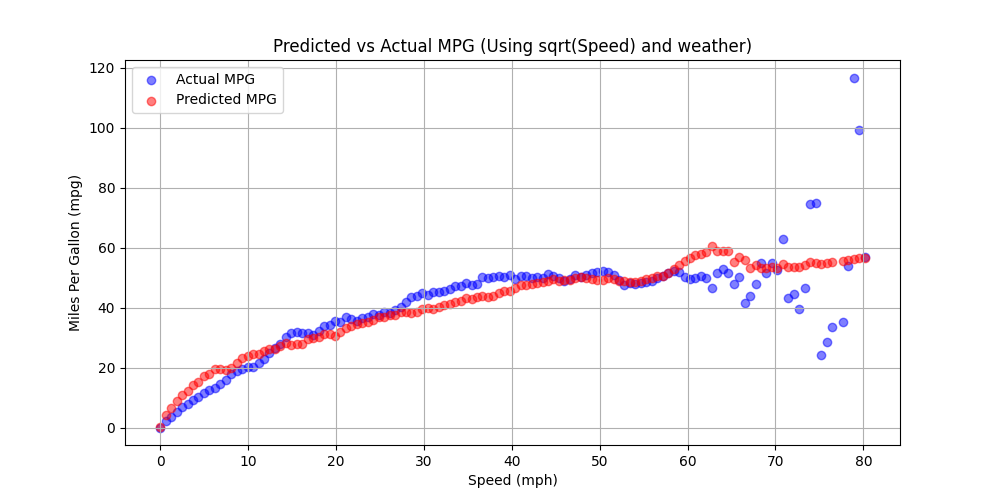
\includegraphics[width=0.5\textwidth]{figures/sqrt_speed_weather_vs_mpg_multiregression_model.png}
    \caption{Plot of MPG predictions of a linear model using speed and weather data.}
    \label{fig:weatherspeedvsmpg}
\end{figure}

% sqrt_speed_rpm_vs_mpg_multiregression_model.png
\begin{figure}[htbp]
    \centering
    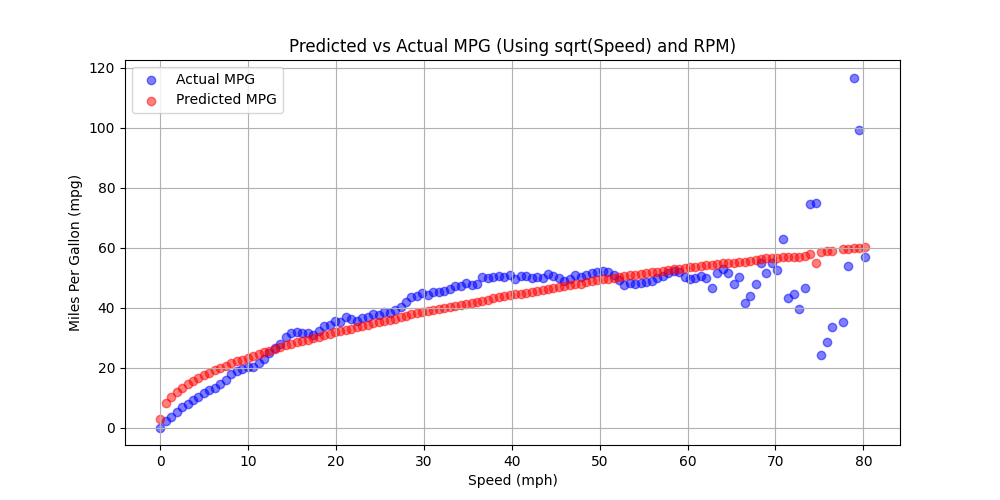
\includegraphics[width=0.5\textwidth]{figures/sqrt_speed_rpm_vs_mpg_multiregression_model.png}
    \caption{Plot of MPG predictions of a linear model using speed and RPM data.}
    \label{fig:rpmspeedvsmpg}
\end{figure}

% speed_vs_mpg_linear_model.png
\begin{figure}[htbp]
    \centering
    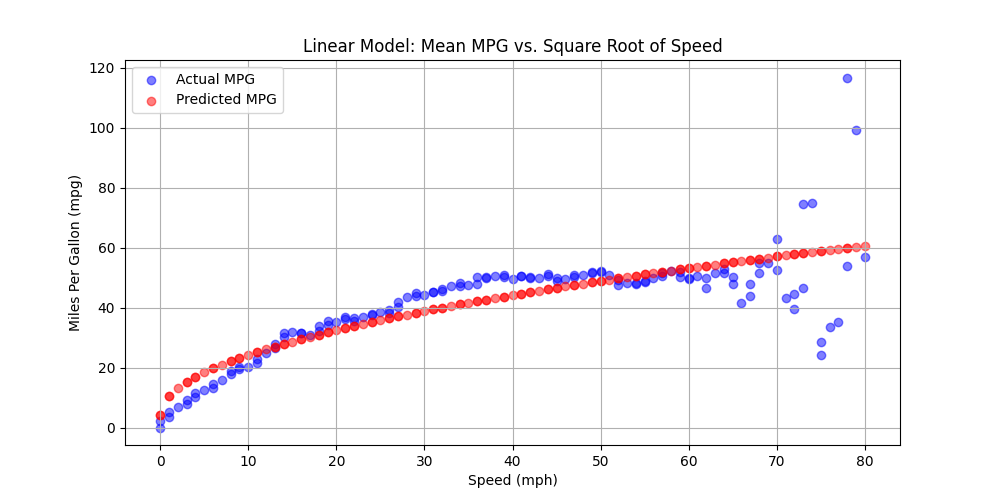
\includegraphics[width=0.5\textwidth]{figures/speed_vs_mpg_linear_model.png}
    \caption{Plot of MPG predictions of a linear model using speed data.}
    \label{fig:speedvsmpglinear}
\end{figure}


\subsection*{LSTM RNN}

\subsubsection*{K-Fold Cross-Validation}

K-fold cross validation was evaluated both on the information extracted 
from the original dataset and the dataset augmented using calculated and 
imported metrics.

An 8-parameter k-fold cross-validation serves as the baseline from which 
other iterations of the algorithm can be evaluated. The parameters used to 
generate this validation were altitude, bearing, air-fuel ratio, engine 
load, engine RPM, intake air temperature, relative throttle position, and 
speed.

\begin{table}[]
    \begin{tabular}{|l|l|l|l|}
        \hline
        \textbf{Layer Num} & \textbf{Hidden Size} & \textbf{$R^{2}$} & \textbf{MAE} \\
        \hline
        2                  & 32                   & 0.4836      & 0.0102       \\
        4                  & 128                  & 0.4662      & 0.0092       \\
        \hline
    \end{tabular}
    \caption{Best-performing models for 8-parameter cross validation.}
    \label{tab:tb1}
\end{table}

The model for this configuration that had the highest $R^{2}$ score had 2 
layers and a hidden layer size of 32, while the model with the lowest MAE 
had 4 layers and 128 nodes in the hidden layers. Performance for these two 
models was generally very similar.

The 9-parameter k-fold cross validation augmented the base case by 
including the outside temperature at the time of driving, in addition to 
the already-existing parameters.

\begin{table}[]
    \begin{tabular}{|l|l|l|l|}
        \hline
        \textbf{Layer Num} & \textbf{Hidden Size} & \textbf{$R^{2}$} & \textbf{MAE} \\
        \hline
        2              	& 64               	& 0.4798  	& 0.0097   	\\
        4              	& 128              	& 0.4542  	& 0.0091 	\\
        \hline
    \end{tabular}
    \caption{Best performing models for 9-parameter cross-validation.}
    \label{tab:tb2}
\end{table}

The better-performing model architectures for the 9-parameter data follow 
a similar pattern to the 8-parameter data. However, in order to achieve an 
optimal $R^{2}$ score, the size of the hidden layer had to be doubled from 
32 to 64. The most likely cause of this is the increased complexity from 
the additional parameter.

The slope grade for a particular interval of the road was added to the 
9-parameter dataset to see how that increased model performance. This 
value was calculated from the change in altitude for a specific interval 
at a given speed.

\begin{table}[]
    \begin{tabular}{|l|l|l|l|}
        \hline
        \textbf{Layer Num} & \textbf{Hidden Size} & \textbf{$R^{2}$} & \textbf{MAE} \\
        \hline
        2              	& 256              	& 0.6227  	& 0.0116   	\\
        4              	& 128              	& 0.5057  	& 0.0102 	\\
        \hline 
    \end{tabular}
    \caption{Best performing models for 9-parameter cross-validation w/ slope grade.}
    \label{tab:tb3}
\end{table}

The best-performing $R^{2}$ results for this permutation of data continue 
to follow the pattern set by the previous model: a drastic increase in 
hidden layer size was required to attain optimal results. Interestingly, 
the increase resulted in a marked improvement in $R^{2}$ compared to the 
difference between the 8-parameter and 9-parameter datasets.

Another interesting thing to note is that the 4-layer 128-hidden-layer-size 
continues to provide the best MAE out of all sizes evaluated. Even though 
both models improved on $R^{2}$, the MAE increased, most likely due to the 
added complexity of the grade parameter.

Because the amount of fuel used is inversely correlated with the fuel 
economy, theoretically one can be calculated if the other is accurately 
predicted by the model. The dataset augmented with weather data and slope 
grade was used to predict only fuel use, and from that, fuel economy was 
calculated.

This configuration resulted in one of the best performing models in all of 
the entire results. The model had 6 layers and a hidden layer size of 64, 
and it was able to obtain both the highest $R^{2}$ score and lowest MAE 
value at 0.8794 and 0.0013, respectively.

The final modification to the dataset tested was removal of the bearing 
parameter. Again, only the fuel use was predicted, and weather data and 
slope grade were included.

\begin{table}[]
\begin{tabular}{|l|l|l|l|}
    \hline
    \textbf{Layer Num} & \textbf{Hidden Size} & \textbf{$R^{2}$} & \textbf{MAE} \\
    \hline
    4              	& 64               	& 0.8234  	& 0.0014   	\\
    6              	& 128              	& 0.8205  	& 0.0014 	\\
    \hline
\end{tabular}
\caption{Best performing models for weather and grade, bearing omitted.}
\label{tab:tb4}
\end{table}

The overall performance of the models in this situation was reduced by a 
noticeable amount. In both models, $R^{2}$ was reduced by about 0.05. MAE 
saw a drop that can be considered inconsequential; approximately 0.0001.

\subsubsection*{Brake-Specific Fuel Consumption}

An alternative model architecture was proposed and implemented in an effort 
to broaden understanding of the target problem. The model implemented a 
RNN with long short-term memory (LSTM) and linearization layers.

The brake-specific fuel consumption (BSFC) was used to estimate fuel 
consumption using the torque, load, and RPM of the engine. These values 
were included as part of an alternative dataset, the POLIDriving dataset.

Training on this data, the model attempted to predict a flow rate in liters 
per hour, which was compared to the value from the BSFC calculation. Over 
the course of 100 epochs, the model was able to successfully learn the fuel 
usage, and it had a total loss at the end of training of 3.0846 
(Figure \ref{fig:lossrnn}).

\begin{figure}[h!]
    \centering
    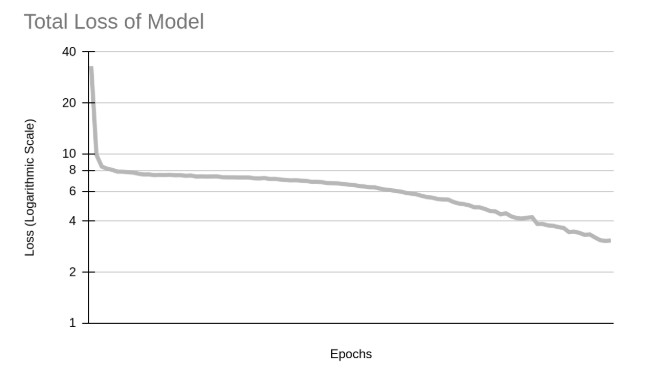
\includegraphics[width=0.5\textwidth]{figures/loss.jpg}
    \caption{Loss of the RNN on the POLIDriving dataset}
    \label{fig:lossrnn}
\end{figure}

When compared against the original data, the model was able to closely 
match the true value (Figure \ref{fig:predictionrnn}).\\

% rnn_predictions.png
\begin{figure}[h!]
    \centering
    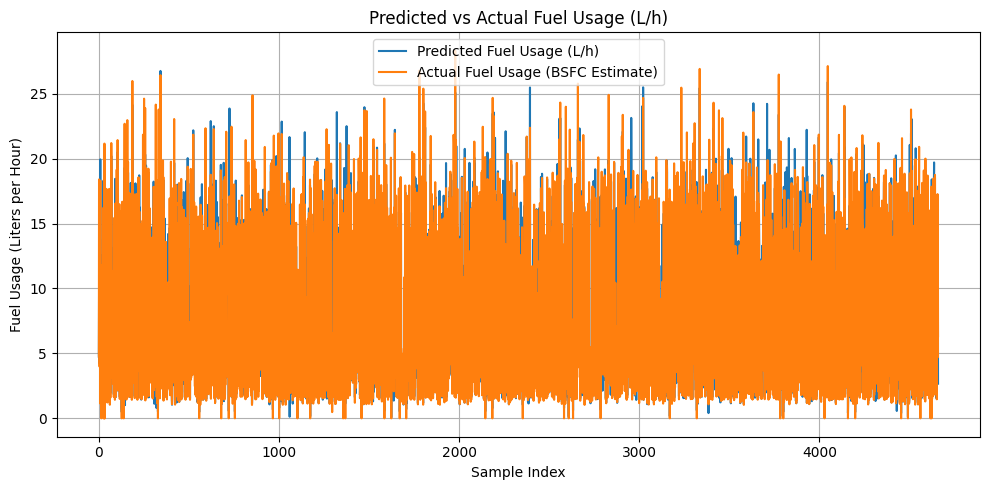
\includegraphics[width=0.5\textwidth]{figures/rnn_predictions.png}
    \caption{Predictions of the RNN on the POLIDriving dataset}
    \label{fig:predictionrnn}
\end{figure}

\subsubsection*{Final Model}

A final model was trained using what was considered to be the best 
combination of parameters and hyperparameters. The number of layers chosen 
was 6, and the size of the hidden layers was 64.

The dataset chosen was the final one evaluated, where bearing was 
included. Again, the amount of fuel used was predicted and fuel economy 
calculated from that.

The overall metrics for the model are as follows:

\begin{table}[h!]
    \begin{tabular}{|l|l|}
        \hline
        Metric & Value \\
        \hline
        MAE          	& 0.00097	\\
        MSE          	& 0.000003   \\
        R2 Score     	& 0.954  	\\
        SAE          	& 552.4384   \\
        SSE          	& 1.8007 \\
        \hline
    \end{tabular}
    \caption{Performance metrics of final model after training.}
    \label{tab:my-table}
\end{table}

Comparing the predicted fuel consumption total against the actual total 
resulted in a total error of 2.8742\%. These results further reinforce the 
conclusion that our proposed ``optimal'' model is well-suited with the 
chosen features extracted from the dataset.

Finally, an analysis of the computational load of this final model was 
carried out using the \verb|fvcore| Python module. On a batch size of 1, 
the model required approximately 1.8 MFLOPS. Modern graphics cards are 
capable of handling orders of magnitude more data, and even the Intel 
i386 microprocessor can run a similar amount of calculations 
(https://www.jcmit.net/cpu-performance.htm).

\end{document}